\documentclass[11pt,a4paper]{report}

% font
%\usepackage{fontspec}
%\setmainfont{Times New Roman}
%\usepackage{tgschola}

\usepackage{helvet}
\renewcommand{\familydefault}{\sfdefault}

\usepackage[margin=0.8in]{geometry}
\usepackage[utf8]{inputenc}
\usepackage{amsmath}
\usepackage{amsfonts}
\usepackage{amssymb}


% https://www.sharelatex.com/learn/Hyperlinks
\usepackage{hyperref}
\hypersetup{
    colorlinks=true,
    linkcolor=red,
    filecolor=magenta,      
    urlcolor=red,
}
 
\usepackage{float}

% https://tex.stackexchange.com/questions/94224/how-to-create-a-list-with-a-fixed-prefix-and-incremental-numbers
\usepackage{enumitem}

\usepackage{lipsum}% http://ctan.org/pkg/lipsum

%% Bibliography/references packages
\usepackage[comma]{natbib}
%%\bibliographystyle{agsm}
\bibliographystyle{dcu}

% CODE
%\usepackage{listings}
%\usepackage{xparse}
%\usepackage{verbatim}
%\NewDocumentCommand{\codeword}{v}{%
%\texttt{\textcolor{blue}{#1}}%
%}
%s\lstset{language=C,keywordstyle={\bfseries \color{blue}}}
\usepackage[outputdir=build]{minted}
\usemintedstyle{vs}

%% https://en.wikibooks.org/wiki/LaTeX/List_Structures
\usepackage{scrextend}

% tables, row colour
\usepackage{tabularx,colortbl}
% For vertical centering text in X column
\renewcommand\tabularxcolumn[1]{m{#1}}

% https://tex.stackexchange.com/questions/22751/how-to-force-table-caption-on-top
%\usepackage[tableposition=top]{caption}
\usepackage{float}
\floatstyle{plaintop}
\restylefloat{table}

% https://en.wikibooks.org/wiki/LaTeX/List_Structures
\usepackage{enumitem}

% https://jansoehlke.com/2010/06/strikethrough-in-latex/
\usepackage{ulem}

%% Report variables
\newcommand{\scname}{PRCO304}
\newcommand{\dlatestv}{2.10}

\definecolor{babyblueeyes}{rgb}{0.63, 0.79, 0.95}
\definecolor{ballblue}{rgb}{0.13, 0.67, 0.8}
\definecolor{beaublue}{rgb}{0.74, 0.83, 0.9}
\definecolor{blue8}{rgb}{0.09, 0.39, 0.67}
\definecolor{blue9}{rgb}{0.00, 0.30, 0.51}
\definecolor{blue9d}{rgb}{0.00, 0.21, 0.36}


%\usepackage{etoolbox}
%\patchcmd{\chapter}{\thispagestyle{plain}}{\thispagestyle{fancy}}{}{}

%https://tex.stackexchange.com/questions/75667/change-colour-on-chapter-section-headings-lyx
\usepackage{sectsty}
\chapterfont{\color{blue9d}}
\sectionfont{\color{blue9d}}
\subsectionfont{\color{blue9d}}
\subsubsectionfont{\color{blue9d}}
%\allchapterfont{\itshape}

\usepackage{titlesec}

\usepackage{array,booktabs,arydshln,xcolor}
\usepackage{xcolor}% http://ctan.org/pkg/xcolor
\usepackage{fancyhdr}% http://ctan.org/pkg/fancyhdr
\fancypagestyle{plain}{%
	\renewcommand{\headrulewidth}{3pt}
	\renewcommand{\headrule}{\hbox to\headwidth{%
		\color{blue9}\leaders\hrule height \headrulewidth\hfill}}
	\renewcommand{\footrulewidth}{3pt}
	\renewcommand{\footrule}{\hbox to\headwidth{%
		\color{blue9}\leaders\hrule height \headrulewidth\hfill}}
	
	%\fancyhf{}
	%\fancyhead[LE]{\textbf{\leftmark}}
	%\fancyhead[RE]{\textbf{\scname{}}}
	%\fancyhead[LO]{\textbf{\scname{}}}
	%\fancyhead[RO]{\textbf{\rightmark}}

	%\fancyfoot[LE]{\textbf{\thepage}}
	%\fancyfoot[RE]{\textbf{\scname{} Configuration Guide}}
	%\fancyfoot[LO]{\textbf{\scname{} Configuration Guide}}
	%\fancyfoot[RO]{\textbf{\thepage}}
}


%% Make bibliography show in table of contents
%% https://tex.stackexchange.com/questions/8458/making-the-bibliography-appear-in-the-table-of-contents
\usepackage[nottoc,numbib]{tocbibind}
%% ^^^ overwrites \bibname, so set it back
\renewcommand{\bibname}{References}

\RequirePackage{filecontents}
\begin{filecontents}{prco304_h4.bib}
@inproceedings{safety_fpga,
  title={FPGAs in critical hardware/software systems},
  author={Hilton, Adrian J and Townson, Gemma and Hall, Jon G},
  booktitle={Proceedings of the 2003 ACM/SIGDA eleventh international symposium on Field programmable gate arrays},
  pages={244--244},
  year={2003},
  organization={ACM}
}
@online{defstan_0056,
	title={Safety Management Requirements for Defence Systems},
	url={https://segoldmine.ppi-int.com/content/standard-def-stan-00-56-safety-management-requirements-defence-systems},
	year={2007}
}
@article{defstan_0056_2,
  title={Safety-critical systems, formal methods and standards},
  author={Bowen, Jonathan and Stavridou, Victoria},
  journal={Software Engineering Journal},
  volume={8},
  number={4},
  pages={189--209},
  year={1993},
  publisher={IET}
}
@article{iec61508,
  title={Introduction to IEC 61508},
  author={Bell, Ron},
  booktitle={Proceedings of the 10th Australian workshop on Safety critical systems and software-Volume 55},
  pages={3--12},
  year={2006},
  organization={Australian Computer Society, Inc.}
}

@misc{scarabhardware,
title={MiniSpartan6+}, 
journal={{Scarab Hardware}},
url={https://www.scarabhardware.com/minispartan6/},
year=2014
}
@misc{arty,
title={Arty Artix-7 FPGA Development Board}, 
journal={{Avnet}},
url={https://uk.rs-online.com/web/p/programmable-logic-development-kits/1346478/},
year=2015
}
@misc{arndt2002algorithms,
  title={Algorithms For Programmers},
  author={Arndt, J{\"o}rg},
  year = 2002
}
@book{hdl,
title={HDL Programming Fundamentals: VHDL and Verilog},
author={Nazeih Botros},
year={2006},
publisher={Da Vinci Engineering Press}
}

@misc{arm, title={ARM in the World of FPGA-Based Prototyping}, url={https://community.arm.com/processors/b/blog/posts/arm-in-the-world-of-fpga-based-prototyping}, journal={Arm Community},
year={2016}}

@book{microblaze,
title={MicroBlaze 
Processor Reference 
Guide},
journal={Xilinx},
year={2017}
} 

\end{filecontents}

%s comments
\usepackage{verbatim}

%inline graphs
\usepackage{wrapfig}
% multiple figures on line
\usepackage{subfig}

\usepackage{graphicx}
\graphicspath{ {img/} }

% Caption font size
% https://tex.stackexchange.com/questions/86120/font-size-of-figure-caption-header
\usepackage[font=scriptsize,labelfont=bf]{caption}

%\setlength{\belowcaptionskip}{-10pt}
%\setlength{\abovecaptionskip}{-5pt} % Chosen fairly arbitrarily


\usepackage{fancyhdr}
\pagestyle{fancy}
\lhead{\rightmark}
\chead{}
%\rhead{FPGA-based RISC Microprocessor and Compiler (Rev. \dlatestv{})}
\rhead{PRCO304 (Rev. \dlatestv{})}
\lfoot{Ben Lancaster 10424877}
\cfoot{}
\rfoot{Page \thepage}

\renewcommand{\subsectionmark}[1]{\markright{\thesubsection\ #1}}


\begin{document}

\makeatletter
\DeclareRobustCommand*{\nameref}{%
\color{blue}%
        \@ifstar\T@nameref\T@nameref
        }%
\makeatother

\begin{titlepage}
\begin{center}

\vspace*{5cm}
\Large

{\color{blue9d}
\textbf{
%%PRCO304 - Project Initiation Document
%Highlight Reports
FPGA-based RISC Microprocessor and Compiler (Rev. \dlatestv{})
}
}

\vspace{0.4cm}
\large
%%Space optimised FPGA-based side-microprocessor.
PRCO304 - Final Stage Computing Project
%%EMBEDDED CPU - FPGA-based RISC microprocessor

\vspace{4cm}
\textbf{Ben Lancaster 10424877}\\
\today 


\end{center}

\end{titlepage}

\pagestyle{plain}

\section*{Revision History}
\begin{table}[h]
\def\arraystretch{1.5}%  1 is the default, change whatever you need
    \begin{tabularx}{\textwidth}{|l|l|X|}
    \hline
    Date & Version & Changes \\
	\specialrule{2pt}{-2pt}{0pt}
	22/03/2018 & 2.10 & Add section \ref{sect:compiler_ast} \nameref{sect:compiler_ast}. \\ \hline
	15/03/2018 & 2.00 & Add section \ref{sect:compiler_grammar} \nameref{sect:compiler_grammar}. \\ \hline
	11/03/2018 & 1.00 & Initial section outline. \\ \hline
    \end{tabularx}
    \caption{Document revisions.}
\end{table}
\newpage


\chapter*{Abstract}
ben

\newpage
\renewcommand*\contentsname{Table of Contents}

{\hypersetup{linkcolor=black}
\tableofcontents
\listoffigures
\listoftables}
 
\newpage

\chapter{Introduction}
Modern computing and electronics equipment, like function generators, oscilloscopes, and spectrum analysers, use FPGAs to implement their compute intensive logic. These FPGAs are often accompanied by a small, low-cost, microprocessor to supervise and provide interfaces to external peripherals.

The aim of this project is to implement this side-microprocessor into the FPGA to save on BOM costs, PCB  space,  and  power  costs,  which  contribute  to  higher  development  and  product  costs.  While  savings can  be  made  by  the  lack  of  side  microprocessor,  the  product  may  need  a  larger  FPGA  to  accommodate the embedded microprocessor.  The project will produce a small, soft-core, CPU design and compiler. Although there is no direct client in this project, I believe this project will produce an attractive product
for FPGA-based product designers wishing to employ an embedded processor solution.

%\lipsum[0-1]

\section{Background}
\subsection{Current Implementations}
\lipsum[0-1]
\newpage

\section{Project Overview}
This project aims to provide an efficient and cost-saving alternative for board and hardware product designers utilising side-microprocessors by designing, implementing, and demonstrating, a small, portable, FPGA processor core design to be used in-place of the side-microprocessor. 

The processor core will implement it's own processor and instruction set architecture and so a compiler and assembler will also be provided so that software code can easily be executed on the processor.

\subsection{Core Deliverables}
These core (C) deliverables are the base requirement for the project to be released in a functional and worthwhile state.
\begin{enumerate}[label=C\arabic*.]
\item{To improve my knowledge and experience of FPGA development, processor architecture, compilers, and embedded systems engineering.}
\item{To build a working and operational soft-core processor core capable of performing simple tasks.}
\item{Implementation of the soft-core processor design on real hardware.}
\item{To provide product designers with an affordable alternative to a side-microprocessor in their FPGA-based products.}
\item{To provide a technical processor reference guide and specification for the embedded core.}
\end{enumerate}

\subsection{Extended Deliverables}
These extended (E) deliverables may not be achievable in the time frame specific in section \ref{sect:proj_time} as they may require extra time to design and implement, require more experience or skill, or require resources currently unattainable.
\begin{enumerate}[label=E\arabic*.]
\item{To provide embedded products a convenient solution to in-field updating.}
\item{To provide easy interfacing between the FPGA design and the embedded core.}
\item{GCC/LLVM/8CC compiler backend for C programming.}\label{sect:deliv:ed:gcc}
\item{Wishbone interface for easier modularity and inter-module communication.}
\item{Multi-core design with Wishbone (2).}
\item{Configurable build options (register/bus widths, optimisations/pipelining, user/privileged mode to support modern operating systems).}
\item{Memory management modules to provide protected and virtual memory lookup tables.}
\end{enumerate}


\newpage
\section{Legal and Ethical Considerations}
\subsection{Privacy}
The \scname{} processor will be able to read and write to all data passing through it and control all connected peripherals (such as UARTs, SDRAMs, and SD Cards). The processor does not track or store usage behaviour, instructions and their frequency,   memory contents, or timing statistics, or any other usage metric.

\subsection{Fit for Purpose}
The \scname{} processor is not designed to run general purpose operating systems, such as Linux or embedded RTOS systems. All memory devices attached to the FPGA are fully accessible to the processor core and instructions/programs running through it, meaning that operating systems or secure applications storing private and sensitive information is not protected by modern processor features such as privilege modes and virtual memory sections. The processor lacks common components required to run modern operating systems, such as a memory management unit (MMU) and privilege modes, and so should not be run on the processor.

The \scname{} processor is not designed to run in high-reliability or safety-critical environments that require established safety standards, such as the UK Defence Standard 00-56 \citep{defstan_0056_2} and IEC 61508 \citep{iec61508}.
\newline\newline
The \scname{} processor, by design, should be used as a replacement for a simple micro-controller accompanying a main processing module.

\subsection{Third-party Libraries}
This project uses only 1 external library for the processor core's universal asynchronous receiver-transmitter (UART) module that does not depend on any other libraries. This allows me to guarantee that: the project rights are secure; and application behaviour is well-defined and predictable (no exploits introduced/injected from external libraries). The UART module does feature a large first-in-first-out (FIFO) buffer for temporary storage of in- and out- going messages. This FIFO is internal to the FPGA design and so is protected from external viewing/modification by probing the board in which the core is running on.

The compiler sub-project does not use any external library dependencies, does not record telemetry or usage statistics, and does not require an internet connection to run.

\subsection{Generated Code}
The code generated by the compiler is \textbf{not guaranteed} to:
\begin{itemize}
\item{\textbf{Produce code for secure environments}. The compiler will not randomise, obfuscate, or split-up and spread, output code. Output machine code will be in a predictable format (global variables in low-memory, instruction memory in middle-memory, and stack memory in high-memory) making the binary easily subject to reverse-engineering and modification.}
\item{\textbf{Produce constant time executable code for expressions}. For example, the compiler output for an \textit{if} statement may implicitly vary depending on it's condition expression, which may have been optimised out, constant-folded, or without-optimisation. This also applies for user code aiming to create reliable and accurate time delay loops; although the processor does not perform optimisations such as instruction caching or branch prediction, access to memory and ALU operations may vary in time, resulting in unreliable instruction times.}

\end{itemize}


\chapter{Project Management}
\section{Time Management}\label{sect:proj_time}
\section{Version Control}
Version control will be utilised to improve work-flow, reference and review code changes, and protect the project from data loss and corruption. GitHub, a git hosting provider, will be utilised to host all project files, including documentation and design files. 

The repository can be found here: \href{https://github.com/bendl/prco304}{https://github.com/bendl/prco304}.

\section{Method of Approach}
Development of the \textbf{core} and \textbf{compiler} will be done in separate stages of the project (see section \ref{sect:proj_time}). The two deliverables will be split into 2 sub-projects. Both sub-projects will employ the \textbf{Agile development process}, using Agile's sprints to split up tasks into sub-tasks and Agile's scrums to discuss progress, features, and changes. This technique allows revisiting of tasks to tweak and iterate over their implementation which will be key when for incrementally adding features to both sub-projects, for example, adding to the core's ALU module to add conditional branching, or adding new instructions to the core's decoder module.

\section{Requirements}
\section{Resources and Dependencies}
For the first half of the development cycle, the core can be developed and verified using the Verilog simulator and test suite, \textbf{Verilator}, and VHDL and Verilog simulator, \textbf{iSim}.

The second half of development will require deploying and debugging on real hardware. This will require an FPGA development kit. To better emulate customer products, the development kit should feature common components such as LEDs, GPIO, USB interface, flash-based storage and memory, and optionally an analogue audio output port. The low-middle range of FPGA devices the project is targeting is the popular and affordable yet feature rich Spartan-6 and Artix-7 FPGAs. From my placement, I have gained experience in Xilinx FPGAs and so will be targeting them for this project to reduce risk and development time.
\\\\
The following FPGA development kits are suitable for this project:
\begin{enumerate}
\item{MiniSpartan6+ - Scarab Hardware - £79 (already owned) \citep{scarabhardware}. The MiniSpartan6+ features a Spartan-6 XC6SLX9 FPGA, 8 LEDs, 2 digital and analogue headers, FT2232 FTDI USB to JTAG, 64Mb SPI flash memory, 32MB SDRAM, an audio output jack, and a MicroSD socket.}

\item{Arty Artix-7 FPGA Development Board - Digilent - £100 \citep{arty}. The Arty development board features a larger Artix-35T FPGA with over 20x the number of logic cells and block memory compared to the LX9 in the MiniSpartan6+. The board components include 256MB DDR3 RAM, 16MBx4 SPI flash memory, USB-JTAG, 8 LEDs (4 of which are RGB), 4 switches, 4 buttons, and multiple Pmod connectors.
\\\\
The greater number of IO options and larger FPGA make the Arty board better suited to emulating real customer products.
}
\end{enumerate}

The project will require a computer or laptop to develop the core and compiler on and continuous integration systems to perform testing on the incremental builds. For the project demo, an oscilloscope (already owned) or digital logic analyser may be required to demonstrate some of the core's features.

\chapter{\scname{} Processor Design}
\section{High Level Design}
The \scname{} processor is a modularised processor with modular logic blocks for the ALU, Registers, RAM, and it's peripherals. 


\begin{figure}[H]
\begin{center}
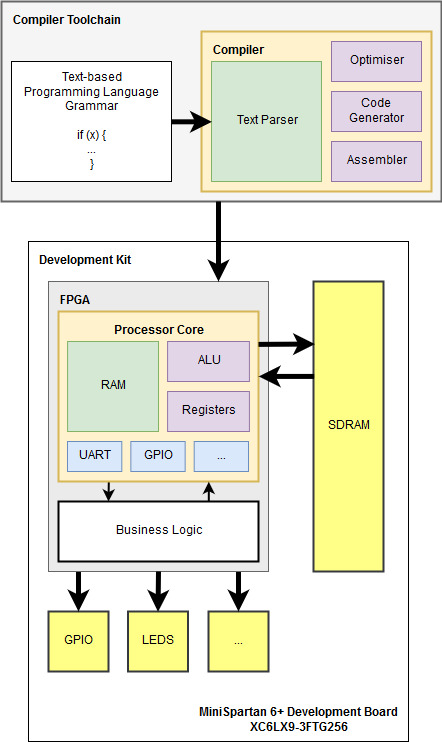
\includegraphics[scale=0.5]{hld}
\end{center}
\caption{test}
\label{fig:hld}
\end{figure}

\section{Registers}
\section{Pipeline Architecture}
\section{Testing and Verification}

\chapter{\scname{} Compiler}
\section{Introduction}
The \scname{} compiler is a command line based software tool used to convert a high-level text grammar (a programming language) into executable machine for the \scname{} processor.

The compiler is invoked with parameters for the input code file and optional parameters specifying optimisation level, target architecture, verbosity, output file name, and include directory paths. The full command line parameter list can be found in {\nameref{sect:compiler_cli}}.


\section{Implementation}
The compiler is implemented fully in the ANSI C programming language due to my familiarity and experience in the language. The compiler is self-contained and requires no dependencies other than the standard C library and CMake to build the project. The project strictly follows the ANSI C89 style guide to make the code more readable.


\section{Text Grammar}\label{sect:compiler_grammar}
The input to the compiler is a generic programming language similar to C.

\begin{minted}{python}
def main() {
    int a = 0;
}
\end{minted}

The grammar is defined below in Backus-Naur Form:
\begin{figure}[H]
\begin{minted}{bnf}
<word>     ::= [a-zA-Z]+[0-9]*
<string>   ::= """ <word> """
<number>   ::= [0-9]+

<top>      ::= <func_def>|<decl>|<extern>

<func_def> ::= <proto><body>
<proto>    ::= "def" <word> "(" <args> ")" 
<body>     ::= "{" <primary> "}"

<primary>  ::= <decl>|<control>|<assign>
<decl>     ::= <word> "=" <expr>

<control>  ::= <if>|<for>|<while>
<if>       ::= "if" "(" <expr> ")" <body>
<for>      ::= "for" "(" <expr> <expr> <expr> ")" <body>

<expr>     ::= <assign>|<binop>|<number>|<string>|"("|")"

<assign>   ::= <word> "=" <expr>
<binop>    ::= "+"|"-"|"*"|"/" <expr>
\end{minted}
\label{fig:compiler_grammar_bnf}
\caption{BNF definition for the input programming language.}
\end{figure}

It should be noted that the grammar and compiler do not have any terminals for defining datatypes, such as "short" and "int". This is because there is only one datatype supported by both compiler and processor. This is due to the complexity required to support different sized datatypes, for example, calculating how many 16-bit words to allocate on the stack for local parameters and accessing them through offsets is difficult and out of scope.

\subsection{Text Parser}
The compiler implements it's own recursive descent parser for the grammar described in \ref{sect:compiler_grammar}. The parser is able to recognise all context free grammars and therefore would be capable of parsing more complete programming languages such as C and Python. 

While parser generators already exist, such as Bison and Java's ANTLR, it was decided to implement the parser by hand using recursive descent principles as a matter of learning rather than ease of use. Although parsing a more complex grammar would easily be more achievable using a parse generator, the overhead of generating compliant assembly for that complex grammar would be too time consuming and is hence out of scope (see extended deliverable \ref{sect:deliv:ed:gcc}).

\subsection{AST Generation}\label{sect:compiler_ast}
The recursive descent parser stores all terminals in the grammar as structures in \textit{ast.h} containing relocatable information about the parsed text and it's future implementation. This AST result of the text parser is the initial immediate representation used by the compiler.

\begin{wrapfigure}{r}{0.4\textwidth}
\begin{minted}{C}
struct ast_func {
    struct ast_proto *proto;
    struct ast_item  *body;
    struct ast_item  *exit;
    struct list_item *locals;
    struct ast_func  *next;
    int    num_local_vars;
};
\end{minted}
\caption{An AST structure representing a parsed function. It contains sub-structures pointing to it's prototype, body, exit statement, and a list of local variables. (\textit{ast.h:63})}
\end{wrapfigure}

\lipsum[1]


\subsection{Optimisation}
The \scname{} compiler can optionally perform simple optimisations, such as unreachable code elimination and constant folding. The optimisations can be controlled by specifying the \verb|-On| parameter to the CLI, where \verb|n| is the level of optimisation.

The techniques used by the optimiser to perform these optimisations are primitive; the optimiser is not given AST information in SSA (static single assignment) form; and because of this limitation, only basic optimisations can be identified.

\subsubsection{Constant Folding}
Constant folding is performed by the optimiser to reduce (fold) expressions that can be identified as constant. This allows the optimiser to replace AST tree structures containing constant values and no dependencies with shorter and simpler AST items. 

For example, the following expression in Figure \ref{fig:constant_fold} can be identified as constant and can be reduced.


\begin{figure}[H]
\centering 
\begin{minipage}{0.4\textwidth}
\begin{minted}{C}
int a = 1 + (2 + 3) * 4;
\end{minted}
\end{minipage}
\caption{An expression suitable for constant folding.}
\label{fig:constant_fold}
\end{figure}
\begin{figure}[H]
\centering 
\begin{minipage}{0.4\textwidth}
\begin{minted}{C}
int a = 1;
int b = 2;
int c = a + b;
\end{minted}
\end{minipage}
\caption{Example of an expression the optimiser cannot identify as constant.}
\label{fig:constant_fold}
\end{figure}

\begin{figure}[H]
%\begin{wrapfigure}{r}{0.6\textwidth}
\begin{center}
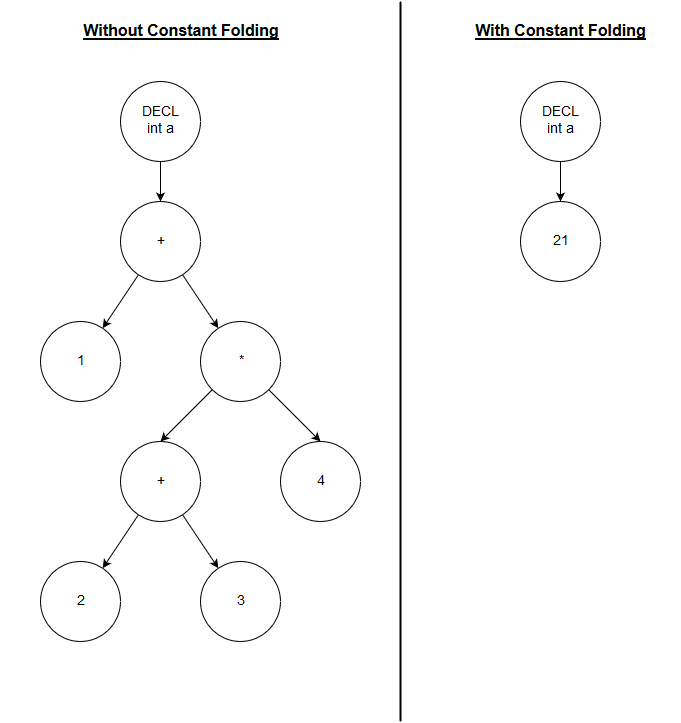
\includegraphics[scale=0.4]{compiler_cf}
\end{center}
\caption{AST transformation performed by Constant Folding.}
\label{fig:compiler_constant_folder}
\end{figure}
%\end{wrapfigure}
%\lipsum[1]
%\lipsum[1]



\subsubsection{Unreachable Code Elimination}
Unreachable code elimination is the removal of code that will never be run on the processor. This can be in the form of uncalled function, unused variables, and control statements that operate on constant values.

The \scname{} compiler can identify some unreachable code segments, such as control statements that operate on constant values, by utilising it's constant folding optimisation discussed previously. By first running the constant folding optimisation on the body of functions, the optimiser looks at the conditions of \textit{for} loop AST items. If their condition has been constant folded to a number and the number is \textit{true} (i.e. not 0) then the AST tree can be replaced with the items in it's body.

\subsection{Code Generation}
The compiler Code Generation stage converts the optimised AST into an intermediatary list of \mintinline{c}{struct prco_op_struct}. It does this by iterating over each \mintinline{c}{struct ast_item} in the AST and checks whether the item requires code generation. For example, an \mintinline{c}{struct ast_item} with type \mintinline{c}{AST_FUNC} is one which requires code generation. The AST is then passed to the \mintinline{c}{void cg_func_prco(...)} function where the code generation takes please. For this type, the stack frame header is generated first, before the body of the body. At the end of the function's body, the stack frame end code generation routing is run.

This code generation stage is named intermediatary because absolute addresses of \verb|JMP| instructions have not been calculated. The calculation of these addresses is performed in the following stage, Assembling. In addition, the location (and offset's) of functions may need to be rearranged.

\subsection{Assembling}
The final stage of the compiler is the assembling stage. This stage takes the list of \verb|struct prco_op_struct| and outputs a list of machine code instructions. The assembler accomplishes this by calculating offsets and addresses of functions, branching instructions, and global variable addresses. It may also rearrange function locations so that the main function is the first instruction to be outputted.

\section{Testing and Verification}
Verifying the output assembly is a bit more involved as there are multiple layers of tests required. The output code generation must be tested for:
\begin{itemize}
\item{(A) Correct machine code output for different code generation routines.}
\item{(B) Correct and complete flow of the output program.}
\end{itemize}
For (A), a code generation routine refers to the code generation function used to produce machine code for a specific structure, for example a function or assignment expression. When machine code instructions are emitted from the code generation routines, they are pushed to a list of \mintinline{c}{struct prco_op_struct} containing information about the emitted instruction. Using this information, the final output machine code word (e.g. \mintinline{c}{0x2020}) is rebuilt into an equivalent \mintinline{c}{struct prco_op_struct} structure and compared against the original. If they are the same, the encoded machine code word is considered correct. This check happens every time an instruction is emitted from the code generation routines.

For (B), two approaches are used. The first is to emit equivalent assembly for another architecture to be compiled are run on the host computer. If the return value of this program is correct, the assembly is assumed to be correct. These tests can be launched by running the \mintinline{bash}{test/run_tests.bat} file. The second approach is to run the compiler output directly on the \scname{} processor, however, this requires rebuilding the FPGA design with the new program code which is time consuming and not always practical.

Another potential solution for verifying output code that is not employed is to create an emulator for the \scname{} processor and have it run the output machine code. This suffers the same problem as (B) where we are relying on systems that may not exactly share the behaviour of the physical processor, be it through unknown bugs, assembly printing errors, or architecture differences.

\chapter{Conclusion}
\section{Project Post-mortem}

\chapter{Appendices}
\section{Appendix A. \scname{} Core Reference Guide}
\section{Appendix B. \scname{} Compiler Reference Guide}
\subsection{CLI Arguments}\label{sect:compiler_cli}

\begin{figure}[H]
\begin{center}
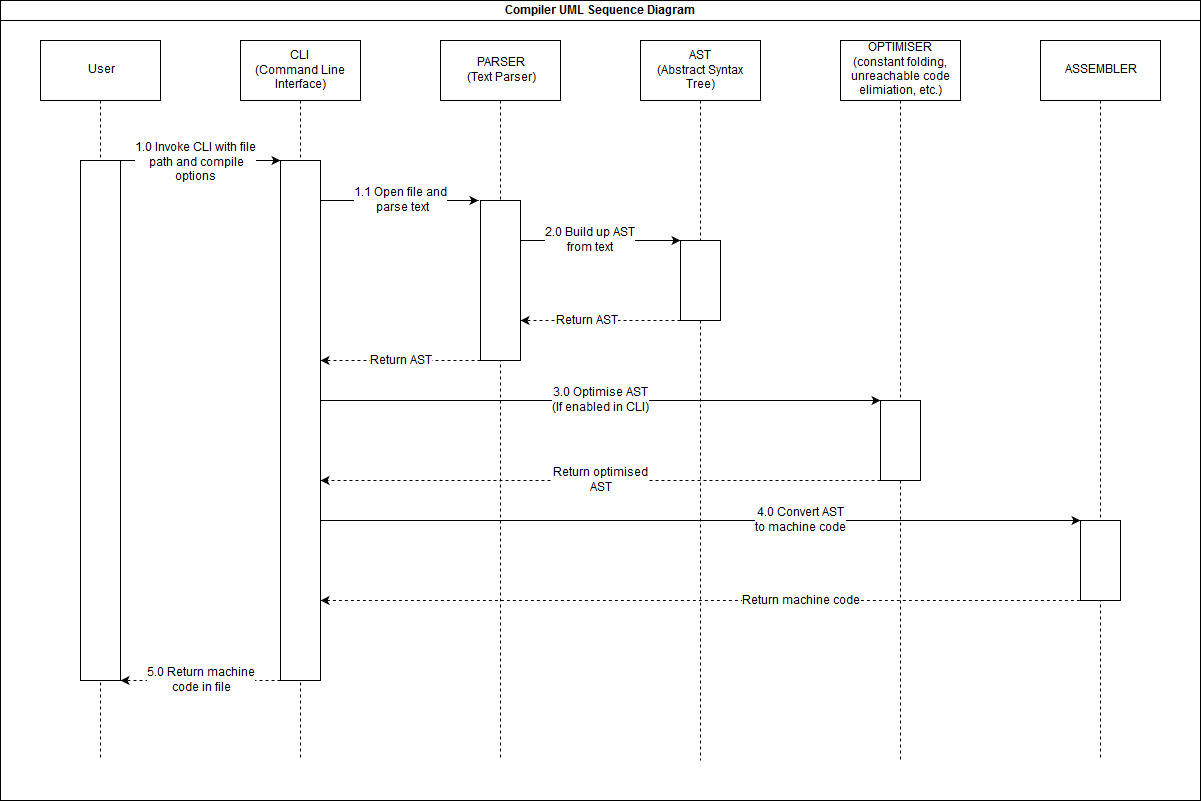
\includegraphics[scale=0.4]{fig_compiler_uml_seq}
\end{center}
\caption{UML sequence diagram for the \scname{} compiler.}
\label{fig:hld}
\end{figure}

\section{Appendix C. Project Initiation Document}

\newpage
\bibliography{prco304_h4} 
\end{document}